\documentclass{article}
\usepackage{iclr2026_conference,times}
\usepackage{graphicx,booktabs,hyperref}
\hypersetup{hidelinks}
\iclrfinalcopy
\title{Separating Evidence Retrieval, Temporal Packing and Conflict-Aware Reading in Agent Memory}
\author{Anonymous Competition Research System}
\begin{document}
\maketitle
\lhead{Competition research manuscript -- no conference submission}
\noindent\textbf{Unreviewed research revision. Previous external scores do not apply.}
\begin{abstract}
Memory-based agents must select admissible evidence and interpret unresolved conflicts under limited context. We implement an auditable workflow that separates temporal filtering of structured records, source packing, and prompted reading. Lexical retrieval, a compact pretrained sentence encoder, and rank fusion provide retrieval baselines. The controlled study shows that preserving competing maximal-time records and interpreting them correctly are complementary: additional verification improves Flash on the versioned controlled arm, whereas Pro already answers that arm correctly with the baseline prompt. Packing outcomes depend on budget and reader, and more context does not improve every condition monotonically. A separate evaluation of the cleaned original LongMemEval corpus compares retrieval policies on matched questions and extends a fixed main arm across the full corpus. Its adapted semantic judge favors lexical over compact dense retrieval for both backbones, while the relative outcome of hybrid fusion depends on the backbone. All registered answer conditions and adapted judgments completed. Historical failed requests still lack measured provider usage and remain covered by explicit admission holds. The contribution is an inspectable evaluation and execution contract, rather than a new temporal model or a claim of general retrieval superiority.
\end{abstract}
\begin{figure}[ht]\centering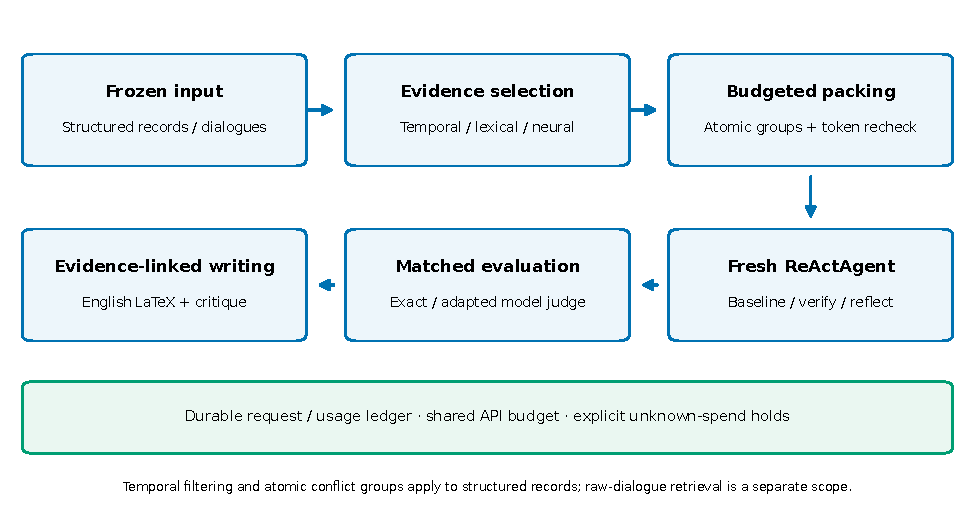
\includegraphics[width=\linewidth]{architecture.pdf}\caption{Implemented research workflow. Temporal filtering and atomic conflict grouping operate on structured records; dialogue passages use a separate retrieval interface. The ledger covers paid answering, adapted judging and writing.}\end{figure}
\section{Introduction}
Long-horizon assistants face distinct questions about memory: which records are admissible at a requested time, which records fit the available context, and how the reader should interpret disagreement among those records. Temporal databases distinguish valid time from the time a fact becomes known \citep{temporal}. Agent memory systems address additional issues such as storage, retrieval, and state updates \citep{memgpt,memzero,amem}. Combining these concerns in a single end-to-end score can obscure whether an answer fails because evidence was omitted or because available evidence was interpreted incorrectly.

We vary retrieval, packing, and reader choices under controlled conditions. The structured branch exposes valid-time and observation-time fields explicitly; it does not require a model to extract them from dialogue. Its baseline prompt already requires abstention for unresolved conflicts, and an additional verification prompt makes the checking procedure more explicit. The dialogue branch evaluates raw-passage retrieval and answering on LongMemEval \citep{longmemeval}, without claiming that structured temporal filtering transfers automatically to free text.

The engineering contribution is a reusable boundary between selected evidence and a fresh model invocation, accompanied by durable accounting, source-bound analysis, and inspectable writing artifacts. We report gains, ties, and failures by condition. Established temporal filtering, packing objectives, and rank fusion are treated as components whose interactions require measurement, rather than as new algorithms.
\section{Related Work}
Temporal database terminology provides the distinction between valid time and transaction or observation time \citep{temporal}. MemGPT, Mem0, and A-MEM investigate memory organization and management for language-model agents \citep{memgpt,memzero,amem}. Our controlled experiment freezes the record store and varies selection and reading; it does not reproduce these systems' complete memory-update workflows.

Conflict-aware retrieval includes richer mechanisms than preserving contradictory records. EvidentialRAG models evidential support and uncertainty, ArbGraph performs graph-based evidence arbitration, and RAMDocs/MADAM-RAG studies retrieval with conflicting evidence \citep{evidentialrag,arbgraph,ramdocs}. Our conflict-aware reader is an additional checking prompt. It implements neither learned evidential fusion nor a claim graph, so these papers provide relevant distinctions rather than reproduced comparison systems. MemFlow studies intent-driven memory orchestration, Verifiable Memory uses local and global verification, and GraphMemory represents reusable strategies in graph-structured memory \citep{memflow,verifiablememory,graphmemory}. EHR-RAG provides a separate example of time-aware retrieval over longitudinal clinical records \citep{ehrrag}; our results do not establish clinical effectiveness.

The local dense baseline uses a compact pretrained MiniLM-family sentence encoder, while hybrid retrieval uses established reciprocal rank fusion \citep{minilm,rrf}. Their original training procedures are not reproduced. LongMemEval supplies the external dialogue corpus evaluated here with normalized lexical scoring and an adapted semantic judge \citep{longmemeval}. Official-evaluator reproduction and interactive online-memory validation remain separate work. Agent Laboratory and AI-Researcher motivate inspectable research workflows \citep{agentlab,airesearcher}; this study evaluates a registered experiment-and-writing workflow, not autonomous hypothesis discovery.
\section{Methods}
The structured selector filters records by entity and requested attributes, excludes records beyond the valid-time and observation-time cutoffs, and retains every record tied at the maximal valid time for each attribute. These tied records form an indivisible group, including competing values and deletions. The no-conflict ablation instead chooses a tied record using observation time and source order. Neither policy directly resolves an answer. No interval-overlap model is implemented.

Packing variants comprise smaller-group-first admission, dynamic programming over an additive surrogate, and aspect-based round-robin admission. The surrogate gives versioned attribute groups unit utility; retrieval-ranked records use reciprocal-rank utility. The diverse variant visits aspect buckets in rounds after ordering candidates by utility. Every variant rechecks the joined text against the actual proxy tokenizer and preserves whole groups. Surrogate optimality does not imply optimality under nonadditive tokenization.

The baseline reader already requires null for unresolved maximal-time conflicts. The conflict-aware prompt adds explicit internal checks of both cutoffs, tied values, and set/delete cases. Reflection adds a separately billed audit of a draft. Repeated invocations are registered as distinct consistency conditions. A fresh ReActAgent executes each model invocation, and the exact-message Rail checks the already selected and packed messages at transport; it bypasses neither retrieval nor packing.

Raw dialogue is handled separately through dated passages, lexical or compact neural ranking, and rank fusion. Provider usage, local preprocessing, proxy context budgets, and unresolved-spend admission holds are distinct accounting scopes.
\subsection{Frozen Protocol}
The frozen protocol defines 100 synthetic tasks: 16 development tasks and 84 held-out tasks, including 72 controlled cases across three new seed namespaces and 12 packing-stress cases. It registers 2770 answer conditions across the requested model aliases. The external corpus contains 500 verified-source LongMemEval questions. A fixed stratified 70-question subset supports matched retrieval and backbone comparisons; a separate hybrid-Flash arm covers the full corpus. External histories are split into 192 cl100k\_base-token passages, while the dense encoder truncates at 256 wordpieces. Selected external contexts are bounded by 1024 proxy tokens. Context budgets differ from billed provider tokens. Responses, reflection and adapted-judge calls are charged to one experiment ledger. Repeated zero-temperature calls are consistency checks, not independent provider sampling seeds.
\section{Evaluation}
The run completed 2770 of 2770 planned answer conditions. The experiment ledger records 3671 calls and 2134370 provider tokens. All planned answer conditions completed with valid adapted judgments. Billing reconciliation remains incomplete: 3 historical failed attempts have unknown provider usage. A conservative 30000-token admission hold was retained; this is an estimate, not measured usage.  The separate full-corpus hybrid-Flash arm completed 500 of 500 questions: normalized exact 17/500, adapted judge 307/500. These are proxy diagnostics, not official benchmark scores.
\begin{figure}[ht]\centering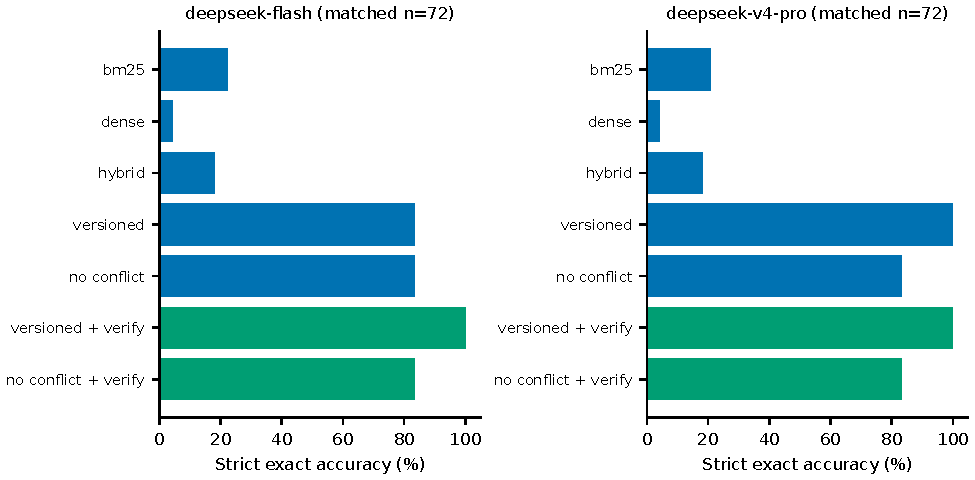
\includegraphics[width=\linewidth]{comparison.pdf}\caption{Common-task synthetic comparison. Exact denominators and task hashes are in the figure manifest.}\end{figure}
\begin{figure}[ht]\centering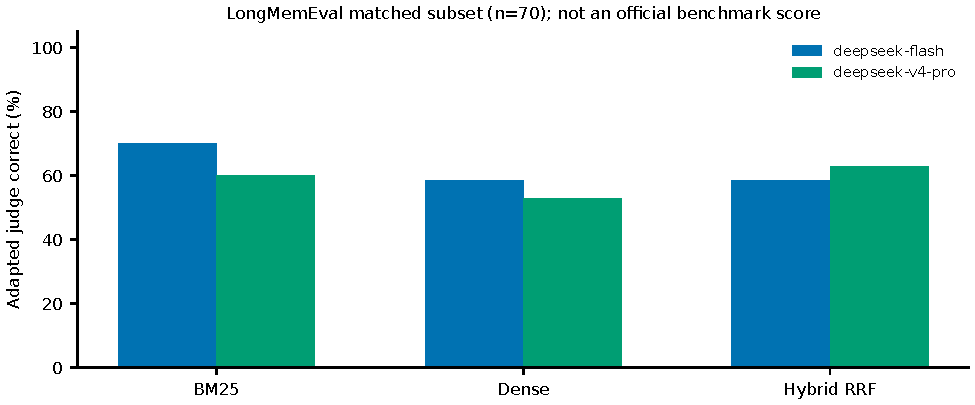
\includegraphics[width=\linewidth]{external.pdf}\caption{Matched external comparison using an adapted DeepSeek judge. This is not an official LongMemEval result.}\end{figure}
\begin{table}[ht]\centering\footnotesize\begin{tabular}{lllrr}\toprule
Model & Policy & Reader & Exact & Judge \\ \midrule
Flash & bm25 & baseline & 16/72 & -- \\
Flash & dense & baseline & 3/72 & -- \\
Flash & hybrid & baseline & 13/72 & -- \\
Flash & no conflict & baseline & 60/72 & -- \\
Flash & no conflict & conflict aware & 60/72 & -- \\
Flash & versioned & baseline & 60/72 & -- \\
Flash & versioned & conflict aware & 72/72 & -- \\
Pro & bm25 & baseline & 15/72 & -- \\
Pro & dense & baseline & 3/72 & -- \\
Pro & hybrid & baseline & 13/72 & -- \\
Pro & no conflict & baseline & 60/72 & -- \\
Pro & no conflict & conflict aware & 60/72 & -- \\
Pro & versioned & baseline & 72/72 & -- \\
Pro & versioned & conflict aware & 72/72 & -- \\
\bottomrule\end{tabular}\caption{Controlled main conditions. Exact task sets and missingness are retained in the report; only matched intersections support paired contrasts.}\end{table}
\begin{table}[ht]\centering\footnotesize\begin{tabular}{lllrr}\toprule
Model & Policy & Reader & Exact & Judge \\ \midrule
Flash & bm25 & baseline & 1/70 & 49/70 \\
Flash & dense & baseline & 0/70 & 41/70 \\
Flash & hybrid & baseline & 1/70 & 41/70 \\
Pro & bm25 & baseline & 0/70 & 42/70 \\
Pro & dense & baseline & 0/70 & 37/70 \\
Pro & hybrid & baseline & 0/70 & 44/70 \\
\bottomrule\end{tabular}\caption{Matched external subset. Exact task sets and missingness are retained in the report; only matched intersections support paired contrasts.}\end{table}
\begin{table}[ht]\centering\footnotesize\begin{tabular}{lllrrr}\toprule
Model & Packer & Reader & Budget 128 & Budget 256 & Budget 512 \\ \midrule
Flash & diverse & baseline & 0/12 & 0/12 & 0/12 \\
Flash & diverse & conflict aware & 0/12 & 0/12 & 12/12 \\
Flash & smaller first & baseline & 0/12 & 8/12 & 0/12 \\
Flash & smaller first & conflict aware & 0/12 & 8/12 & 12/12 \\
Flash & utility dp & baseline & 0/12 & 8/12 & 0/12 \\
Flash & utility dp & conflict aware & 0/12 & 8/12 & 12/12 \\
Pro & diverse & baseline & 0/12 & 0/12 & 10/12 \\
Pro & diverse & conflict aware & 0/12 & 0/12 & 12/12 \\
Pro & smaller first & baseline & 0/12 & 8/12 & 10/12 \\
Pro & smaller first & conflict aware & 0/12 & 8/12 & 12/12 \\
Pro & utility dp & baseline & 0/12 & 8/12 & 11/12 \\
Pro & utility dp & conflict aware & 0/12 & 8/12 & 12/12 \\
\bottomrule\end{tabular}\caption{Packing-stress outcomes across source budgets. Cells show exact-correct/completed on the same registered stress tasks; budgets do not create independent task samples.}\end{table}
\section{Uncertainty and Reproducibility}
Primary comparisons use repeat-zero shared tasks. Repeated answers never inflate task counts. Task bootstrap intervals, exact paired binomial diagnostics and Holm family adjustments are reported as descriptive diagnostics. Shared generators, task families and external conversations leave independence assumptions unverified; no significance or generalization claim is granted.
\begin{table}[ht]\centering\footnotesize\begin{tabular}{p{0.46\linewidth}lrrl}\toprule
Contrast and condition & Model & Paired & $\Delta$ pp & Descriptive interval \\ \midrule
conflict aware vs baseline (exact, B256) & Flash & 72 & +16.7 & [+8.3, +25.0] \\
conflict aware vs baseline (exact, B256) & Pro & 72 & +0.0 & [+0.0, +0.0] \\
versioned vs no conflict (exact, B256) & Flash & 72 & +16.7 & [+8.3, +25.0] \\
versioned vs no conflict (exact, B256) & Pro & 72 & +16.7 & [+8.3, +25.0] \\
bm25 vs dense (external judge, B1024) & Flash & 70 & +11.4 & [-1.4, +24.3] \\
bm25 vs dense (external judge, B1024) & Pro & 70 & +7.1 & [-4.3, +18.6] \\
bm25 vs hybrid (external judge, B1024) & Flash & 70 & +11.4 & [+0.0, +22.9] \\
bm25 vs hybrid (external judge, B1024) & Pro & 70 & -2.9 & [-12.9, +7.1] \\
smaller first vs utility dp (exact, B128) & Flash & 12 & +0.0 & [+0.0, +0.0] \\
smaller first vs utility dp (exact, B128) & Pro & 12 & +0.0 & [+0.0, +0.0] \\
smaller first vs utility dp (exact, B256) & Flash & 12 & +0.0 & [+0.0, +0.0] \\
smaller first vs utility dp (exact, B256) & Pro & 12 & +0.0 & [+0.0, +0.0] \\
smaller first vs utility dp (exact, B512) & Flash & 12 & +0.0 & [+0.0, +0.0] \\
smaller first vs utility dp (exact, B512) & Pro & 12 & -8.3 & [-25.0, +0.0] \\
smaller first vs diverse (exact, B128) & Flash & 12 & +0.0 & [+0.0, +0.0] \\
smaller first vs diverse (exact, B128) & Pro & 12 & +0.0 & [+0.0, +0.0] \\
smaller first vs diverse (exact, B256) & Flash & 12 & +66.7 & [+41.7, +91.7] \\
smaller first vs diverse (exact, B256) & Pro & 12 & +66.7 & [+41.7, +91.7] \\
smaller first vs diverse (exact, B512) & Flash & 12 & +0.0 & [+0.0, +0.0] \\
smaller first vs diverse (exact, B512) & Pro & 12 & +0.0 & [-25.0, +25.0] \\
128 vs 256 (exact, source budgets) & Flash & 24 & +0.0 & [+0.0, +0.0] \\
256 vs 512 (exact, source budgets) & Flash & 24 & +0.0 & [+0.0, +0.0] \\
128 vs 512 (exact, source budgets) & Flash & 24 & +0.0 & [+0.0, +0.0] \\
\bottomrule\end{tabular}\caption{Descriptive paired differences, left minus right, in percentage points. Rows follow fixed condition rules rather than effect size. Task-bootstrap intervals do not establish population coverage or equivalence; full contrasts, task hashes, exclusions and multiplicity diagnostics are in the analysis artifact.}\end{table}
\section{Discussion}
The controlled comparisons support a conditional interaction between evidence selection and prompted verification. Flash improves with the explicit conflict-verification prompt when the versioned selector retains competing maximal-time records; Pro already reaches the observed ceiling in that controlled baseline arm. Removing competing records lowers controlled mechanism accuracy for both backbones, and prompting cannot reliably recover evidence that was discarded. These findings do not imply that verification is universally beneficial or that the structured task proves successful temporal extraction from dialogue.

Packing results depend materially on the source budget. At the smallest tested budget, the stress conditions do not yield complete exact answers. At the intermediate budget, smaller-first and dynamic packing outperform diverse admission. At the largest budget, conflict-aware reading benefits both models, while the packers are mostly tied and a small Pro baseline difference remains. Flash baseline performance can decline as the budget increases. Because packers alter selected evidence as well as ordering, these observations do not isolate an ordering effect or establish distraction as a cause.

External lexical exact matching and adapted semantic judgments measure different properties. The adapted judge favors BM25 over the compact dense baseline for both backbones, while hybrid fusion relative to BM25 changes direction across backbones. This does not establish general inferiority of neural retrieval: the encoder is compact, quantized, and truncated, and the selected context is narrow. The judge also belongs to the evaluated model family.

All registered answers and adapted judgments are complete. Billing reconciliation remains incomplete for historical failures. Paired tests, multiplicity adjustments, and task-bootstrap intervals are available as diagnostics, but shared generators and conversations leave independence assumptions unverified; no significance claim follows.
\section{Conclusion}
This study separates admissible-evidence selection, budgeted packing, and conflict-aware reading within an auditable agent workflow. The controlled mechanism comparison shows complementary roles for retaining conflicting records and checking them explicitly: Flash benefits from additional verification, while Pro already succeeds in the corresponding versioned baseline arm. The no-conflict ablation has lower accuracy for both backbones in that comparison. Packing outcomes change with budget and reader and do not support a universally superior packing method.

The cleaned original LongMemEval corpus was evaluated through raw-passage retrieval, normalized lexical scoring, and adapted semantic judgments. Its matched comparisons do not show universal gains from the compact dense or hybrid baselines, and the full-corpus main arm is reported separately. These are local evaluation results rather than official benchmark scores. All planned answers and judgments completed, while historical provider usage remains unreconciled under conservative admission holds. Stronger retrievers, independent judges, interactive memory updates, and free-text temporal extraction require further evaluation. Established temporal modeling and rank fusion are not claimed as novel, and reviewer acceptance is not inferred from implementation or internal checks.
\section{Limitations}
Temporal modeling and knapsack/RRF mechanisms are established prior art; no novelty claim. External exact/F1 are lexical proxies; a DeepSeek semantic judge is an adapted evaluator, not the official benchmark judge. Repeated zero-temperature calls do not establish independent provider sampling seeds. Neural passages are truncated to 256 wordpieces; proxy context tokens differ from provider billing. Session-level evidence recall does not imply answer-bearing turns survived passage selection. Synthetic families remain related; task-cluster intervals are descriptive, not adjusted significance tests. Semantic judgments by a DeepSeek model may favor related-model answers. The compact quantized encoder is a resource-constrained baseline, not a frontier retriever; stronger embeddings, rerankers and external context-budget sweeps remain untested. The bitemporal selector is assessed on explicit structured records; raw external passage retrieval does not establish successful free-text bitemporal extraction. Audited operational repairs handled Unicode JSONL boundaries and literal reserved-token spellings in source text, with original responses and measured usage retained. Previously accepted source text keeps the same tokenization; newly supported reserved spellings are encoded as ordinary text. Local CPU embedding and API usage are separate resource scopes. Scientific novelty and reviewer acceptance remain unestablished.
\begin{thebibliography}{99}
\bibitem[Jensen et al.(1994)]{temporal} Christian S. Jensen et al. (1994). A Consensus Glossary of Temporal Database Concepts. \url{https://www2.cs.arizona.edu/~rts/pubs/SIGMODRecordMarch94p52.pdf}.
\bibitem[Packer et al.(2023)]{memgpt} Charles Packer et al. (2023). MemGPT: Towards LLMs as Operating Systems. \url{https://arxiv.org/abs/2310.08560}.
\bibitem[Chhikara et al.(2025)]{memzero} Prateek Chhikara et al. (2025). Mem0: Building Production-Ready AI Agents with Scalable Long-Term Memory. \url{https://arxiv.org/abs/2504.19413}.
\bibitem[Xu et al.(2025)]{amem} Wujiang Xu et al. (2025). A-MEM: Agentic Memory for LLM Agents. \url{https://arxiv.org/abs/2502.12110}.
\bibitem[Wu et al.(2024)]{longmemeval} Di Wu et al. (2024). LongMemEval: Benchmarking Chat Assistants on Long-Term Interactive Memory. \url{https://arxiv.org/abs/2410.10813}.
\bibitem[Schmidgall et al.(2025)]{agentlab} Samuel Schmidgall et al. (2025). Agent Laboratory: Using LLM Agents as Research Assistants. \url{https://arxiv.org/abs/2501.04227}.
\bibitem[Tang et al.(2025)]{airesearcher} Jiabin Tang et al. (2025). AI-Researcher: Autonomous Scientific Innovation. \url{https://arxiv.org/abs/2505.18705}.
\bibitem[Hossain et al.(2026)]{evidentialrag} S M Asif Hossain; Ruksat Khan Shayoni; M. F. Mridha (2026). EvidentialRAG: Quantifying and Mitigating Information Conflict in Multi-Source Retrieval-Augmented Generation via Evidential Deep Learning. \url{https://arxiv.org/abs/2607.10491}.
\bibitem[Niu et al.(2026)]{arbgraph} Qingying Niu; Yuhao Wang; Ruiyang Ren; Bohui Fang; Wayne Xin Zhao (2026). ArbGraph: Conflict-Aware Evidence Arbitration for Reliable Long-Form Retrieval-Augmented Generation. \url{https://arxiv.org/abs/2604.18362}.
\bibitem[Chen et al.(2026)]{memflow} Jiayi Chen; Yingcong Li; Guiling Wang (2026). MemFlow: Intent-Driven Memory Orchestration for Small Language Model Agents. \url{https://arxiv.org/abs/2605.03312}.
\bibitem[Sun et al.(2026)]{verifiablememory} Xiaolong Sun; Qichao Wang; Hangyu Li; Liang Chen (2026). Verifiable Memory: Learning Unified Memory Management with Local and Global Verifiers for Large Language Model Agents. \url{https://arxiv.org/abs/2608.03137}.
\bibitem[Farhat et al.(2026)]{graphmemory} Yehya Farhat; Michael Desmond; Anastasios Kyrillidis (2026). Decoupling Memory from Context: Structured Memory for Token-Efficient Test-Time Continual Learning. \url{https://arxiv.org/abs/2610.02687}.
\bibitem[Wang et al.(2025)]{ramdocs} Han Wang; Archiki Prasad; Elias Stengel-Eskin; Mohit Bansal (2025). Retrieval-Augmented Generation with Conflicting Evidence. \url{https://arxiv.org/abs/2504.13079}.
\bibitem[Cao et al.(2026)]{ehrrag} Lang Cao; Qingyu Chen; Yue Guo (2026). EHR-RAG: Bridging Long-Horizon Structured Electronic Health Records and Large Language Models via Enhanced Retrieval-Augmented Generation. \url{https://arxiv.org/abs/2601.21340}.
\bibitem[Wang et al.(2020)]{minilm} Wenhui Wang; Furu Wei; Li Dong; Hangbo Bao; Nan Yang; Ming Zhou (2020). MiniLM: Deep Self-Attention Distillation for Task-Agnostic Compression of Pre-Trained Transformers. \url{https://arxiv.org/abs/2002.10957}.
\bibitem[Cormack et al.(2009)]{rrf} Gordon V. Cormack; Charles L. A. Clarke; Stefan Buettcher (2009). Reciprocal rank fusion outperforms condorcet and individual rank learning methods. \url{https://doi.org/10.1145/1571941.1572114}.
\end{thebibliography}
\end{document}
